\chapter{Related Work} 
This section discusses 4 existing visualisations that have a theme revolving
around
space or planets. Following a short description, each visualisation is analysed
to
discover which of the User Scenarios detailed in the previous chapter exist
within the
system.

\section{Worlds: The Kepler Planet Candidates - Non Interactive}
Worlds \cite{worlds} displays planet candidates found by NASA's Kepler
mission. These candidates are animated in orbit around a single star. They are
drawn to scale with accurate radii, orbital periods, and orbital distances. They
range in size from 1/3 to 84 times the radius of Earth. Colors represent an
estimate of temperature with red indicating warmest, and blue indicating coldest
candidates. 
\begin{figure}[H]
  \centering
      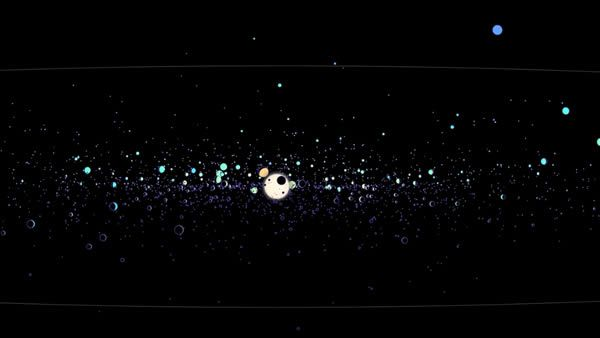
\includegraphics[width=0.8\textwidth]{images/worlds.jpg}
  \caption{Image of Worlds Visualisation}
\end{figure}
Worlds has a visually appealing layout that effectively displays the basic
attributes of each planet. By examining this visualisation we can see how
displaying the planets orbiting a single star allows users to visually make a
basic comparison between each planet. The below paragraphs discuss the User
Scenarios that Worlds fulfills.
 \\\\
{\bf Scenario 1. View planets ordered by their similarity to Earth:\\}
Worlds has comprehensive functionality for comparing the different exoplanets to
one another, however it does not offer any functionality regarding comparisons
to earth 
\\\\
{\bf Scenario 2. Select ranges for attributes of each planet displayed:\\}
Worlds doesn't offer any functionality for any filtering of exoplanets, this
means that users can only see all planets at once which can be overwhelming and
causes exoplanets to be excluded from view due to overlapping
and clustering. The reason that this is done is to convey how many exoplanets
there are and how their scale differs among on another.
\\\\
{\bf Scenario 3. Select planets to display more information:\\}
Worlds is non interactive meaning that users are not able to request further
information about the visualisation elements that they are seeing. This ability
to find out more is a key part of the interactive visualization needed
for this project.

\section{The Kepler Orrery and The Kepler Orrery 2 - Non interactive}
The Kepler Orrery \cite{orrery} illustrates exoplanets in their
own solar systems. The orbit radii are to scale with respect to each other and
planet sizes are to scale with respect to each other, but orbits and planet
sizes are different scales. The colors are in order of semi-major axis:
two-planet systems (242 in all) have a yellow outer planet; 3-planet (85) green,
4-planet (25) light blue, 5-planet (8) dark blue, 6-planet (1, Kepler-11)
purple. 
\begin{figure}[H]
  \centering
      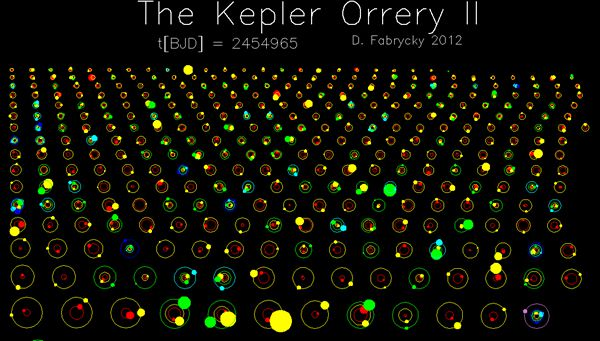
\includegraphics[width=0.8\textwidth]{images/orrery.jpg}
  \caption{Image of The Kepler Orrery Visualisation}
\end{figure}
This system exhibits small multiples, a grid of small similar graphics or
charts, allowing them to be easily compared. This provides insights into how I
can use small multiples to display information about groups of planets. This
will be important for displaying which planets share a solar system. The below
paragraphs discuss the User Scenarios that The Kepler Orrery fulfills.
\\\\
{\bf Scenario 1. View planets ordered by their similarity to Earth:\\}
Like Worlds, The Kepler Orrery shows the similarities between each of the
exoplanets but does not have the functionality to allow users to make a
comparison to earth and our own solar system.
\\\\
{\bf Scenario 4. View planets in the same solar system:\\}
The layout of the visualisation uses small multiples to group each solar system
of exoplanets and stars together which removes the issue of overcrowding and
overlapping elements. Displaying each exoplanet
orbiting its own star removes the risk of confusion about what planets are
actually orbiting which could be the case with Worlds.

\section{Celestia - Interactive}
Celestia \cite{celestia} is a 3D space simulation written in C++. Celestia does
not include any stars that are more than a
few thousand light-years from the Sun because the distant
stars are too small difficult to measure, meaning that it doesn't contain
the distant exoplanets discovered by the Kepler mission. 
\begin{figure}[H]
  \centering
      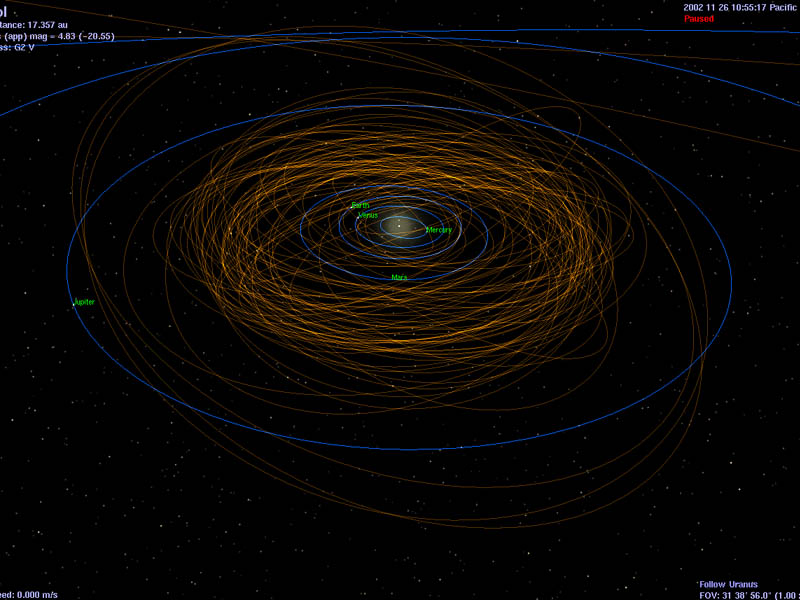
\includegraphics[width=0.8\textwidth]{images/celestia.jpg}
  \caption{Image of Celestia Visualisation}
\end{figure}
This visualisation is much larger and more encompassing system than is needed
for this project, as it is a full simulation. However is does offer
insights into how to effectively portray planets and their orbits (See Figure
2.3). It also provides textures that can be used to depict
what planets look like to increase user immersion. The below paragraphs discuss
the User Scenarios that Celestia fulfills.

{\bf Scenario 3. Select planets to display more information:\\}
Celestia allows users to view a large set of information about each of the
planets that it displays. The information is available in toolbars
that can be accessed. Examples of this information are radius, phase angle,
rotation speed, and temperature of planets.  
\\\\
{\bf Scenario 4. View planets in the same solar system:\\}
Celestia allows users to explore a range of solar systems their planets. This is
a key feature of the experience that
Celestia tries to give users, ie letting them explore the vastness of space in a
3D simulation. 

\section{Kepler Visualisation Tool}
\label{sec:kep}
The Kepler Visualisation tool \cite{kepler_github, kepler_article} is a 3D
visualisation built with Processing (A Java library and development
environment). It is a simple visualisation focusing
on displaying the estimated size, orbital speed, and orbital
separation of each exoplanet. All exoplanets are color-coded to visually
represent
their estimated temperatures.
\begin{figure}[H]
  \centering
      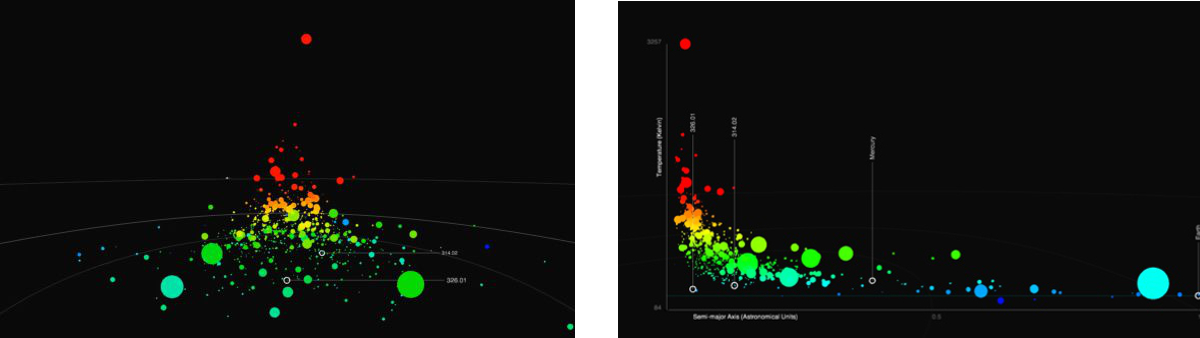
\includegraphics[width=1\textwidth]{images/kepler.jpg}
  \caption{Kepler Visualisation Tool Orbital View}
\end{figure}

The existing work in this system would serve as foundation for this project as
much of the visual aspects, and initial data manipulation of this visualisation
is already complete. It means that implementing the features
needed for this project could be focused on more heavily, and larger
improvements could be undertaken. The below paragraphs
discuss the User Scenarios that Kepler Visualisation Tool fulfills.
\\\\
{\bf Scenario 1. View planets ordered by their similarity to Earth:\\}
Like Worlds and the Kepler Orrery, The Kepler Visualisation Tool has
functionality to display the similarity of each Exoplanet to each other.
However, it also has some limited functionality of comparing these to earth
which the others lack. It does this by displaying Earth, Mars, and Jupiter by
the same method as the Exoplanets. This gives users a point of common reference
with which to make comparisons.
\\\\
{\bf Scenario 2. Select ranges for attributes of each planet displayed:\\}
The Kepler Visualisation Tool allows users to sort the exoplanets on the Y axis
by their size and temperature, but does not allow users to specifiy ranges of
these to filter them.
\section{Summary of Existing Applications}
\begin{figure}[H]
  \centering
      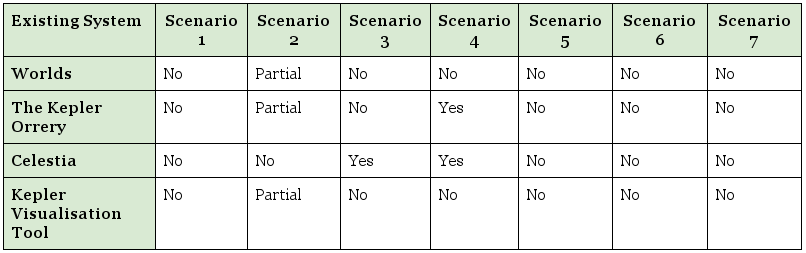
\includegraphics[width=1\textwidth]{images/existing.png}
  \caption{Matrix of existing solutions mapped to scenarios}  
    \label{fig:existing}
\end{figure}


